\documentclass[
	% -- opções da classe memoir --
	12pt,				% tamanho da fonte
	openright,
	oneside,			% para impressão em verso e anverso. Oposto a oneside
	a4paper,			% tamanho do papel. 
	% -- opções da classe abntex2 --
	chapter=TITLE,		% títulos de capítulos convertidos em letras maiúsculas
	%section=TITLE,		% títulos de seções convertidos em letras maiúsculas
	%subsection=TITLE,	% títulos de subseções convertidos em letras maiúsculas
	%subsubsection=TITLE,% títulos de subsubseções convertidos em letras maiúsculas
	% -- opções do pacote babel --
	brazil				% o último idioma é o principal do documento
	]{abntex2}

% ---
% Pacotes básicos 
% ---
\usepackage{lmodern}			% Usa a fonte Latin Modern			
\usepackage[T1]{fontenc}		% Selecao de codigos de fonte.
\usepackage[utf8]{inputenc}		% Codificacao do documento (conversão automática dos acentos)
\usepackage{lastpage}			% Usado pela Ficha catalográfica
\usepackage{indentfirst}		% Indenta o primeiro parágrafo de cada seção.
\usepackage{color}				% Controle das cores
\usepackage{graphicx}			% Inclusão de gráficos
\usepackage{microtype} 			% para melhorias de justificação
\usepackage{float}
% ---
		
% ---
% Pacotes adicionais, usados apenas no âmbito do Modelo Canônico do abnteX2
% ---
\usepackage{lipsum}				% para geração de dummy text
% ---

\usepackage{tabularx} % in the preamble

% ---
% Pacotes de citações
% ---
\usepackage[brazilian,hyperpageref]{backref}	 % Paginas com as citações na bibl
\usepackage[alf]{abntex2cite}	% Citações padrão ABNT


% ---
% Informações de dados para CAPA e FOLHA DE ROSTO
% ---
\titulo{Documento de Requisitos:\\ Controle de prestação de serviço - Any@Bike}
\autor{UNIVERSIDADE ESTADUAL DO MATO GROSSO DO SUL\\ CURSO DE CIÊNCIA DA COMPUTAÇÃO}
\local{Dourados}
\data{Junho de 2015}
\instituicao{Responsável pelo Projeto:\par Felipe Lima Morais}

% O preambulo deve conter o tipo do trabalho, o objetivo, 
% o nome da instituição e a área de concentração 
\preambulo{Trabalho acadêmico apresentado à disciplina de Análise e Projeto de Sistemas, do curso de Bacharelado em Ciência da Computação como requisito parcial para obtenção da nota do segundo bimestre.\newline \newline Profa. Dra. Glaucia Gabriel Sass}
% ---

% alterando o aspecto da cor azul
\definecolor{blue}{RGB}{0,0,0}

% informações do PDF
\makeatletter
\hypersetup{
     	%pagebackref=true,
		pdftitle={\@title}, 
		pdfauthor={\@author},
    	pdfsubject={\imprimirpreambulo},
	    pdfcreator={LaTeX with abnTeX2},
		pdfkeywords={abnt}{latex}{abntex}{abntex2}{trabalho acadêmico}, 
		colorlinks=true,       		% false: boxed links; true: colored links
    	linkcolor=blue,          	% color of internal links
    	citecolor=blue,        		% color of links to bibliography
    	%filecolor=magenta,      		% color of file links
		urlcolor=blue,
		bookmarksdepth=4
}
\makeatother
% --- 

% --- 
% Espaçamentos entre linhas e parágrafos 
% --- 

% O tamanho do parágrafo é dado por:
\setlength{\parindent}{1.3cm}

% Controle do espaçamento entre um parágrafo e outro:
\setlength{\parskip}{0.2cm}  % tente também \onelineskip

% ---
% compila o indice
% ---
\makeindex							%TODO
% ---

% ----
% Início do documento
% ----
\begin{document}

% Seleciona o idioma do documento (conforme pacotes do babel)
%\selectlanguage{english}
\selectlanguage{brazil}

% Retira espaço extra obsoleto entre as frases.
\frenchspacing 

% ----------------------------------------------------------
% ELEMENTOS PRÉ-TEXTUAIS
% ----------------------------------------------------------
% \pretextual

% ---
% Folha de rosto
% (o * indica que haverá a ficha bibliográfica)
% ---
\imprimirfolhaderosto
% ---

% ---
% inserir o sumario
% ---
\pdfbookmark[0]{\contentsname}{toc}
\tableofcontents*
\cleardoublepage
% ---


% ----------------------------------------------------------
% ELEMENTOS TEXTUAIS
% ----------------------------------------------------------
\textual


% ---
% inserir lista de ilustrações
% ---
\pdfbookmark[0]{\listfigurename}{lof}
\addcontentsline{toc}{chapter}{Lista de Figuras}
\listoffigures*
\cleardoublepage
% ---

% ---
% inserir lista de abreviaturas e siglas
% ---
\addcontentsline{toc}{chapter}{Lista de Abreviaturas e siglas}
\begin{siglas}
  \item[CPF] Cadastro de pessoa física 
  \item[RF] Requisitos Funcionais
  \item[RNF] Requisitos Não Funcional
  \item[RU] Requisitos de Usuário
  
\end{siglas}
% ---


\addcontentsline{toc}{chapter}{Prefácio}

\chapter*{Prefácio}

Este documento visa esclarecer e propor o desenvolvimento de sistema para o controle dos atendimentos para concerto de bicicletas da AnyBike.LTDA. Representada neste processo pelo proprietário Juvenal Maresia Antão. O Sr. Juvenal será o intermediador entre a equipe de desenvolvimento e a empresa. 

Versão deste documento: v 1.1

\section*{Versão revisada anterior}
\begin{flushleft}
	\begin{tabular}{| p{3cm} | p{9cm} | p{3cm} |}
 	   \hline
	    \textbf{Versão} 		& \textbf{Comentário} 				& \textbf{Data}  \\ \hline
	    1.0		 				& Primeira versão do documento de %
	    						requisitos estudado e corrigido %
	    						resultando nesta versão. 			& 22/04/2015 		 \\ \hline 	   
	\end{tabular}
\end{flushleft}


\section*{Aprovação do documento}
\begin{flushleft}
	\begin{tabular}{| p{3cm} | p{7cm} | p{5cm} |}
 	   \hline
	    \textbf{Data} 		& \textbf{Nome} 										& \textbf{Assinatura}  \\ \hline
	    23/06/2015	 			& Felipe Lima Morais - gerente do projeto 			& 		 		 		\\ \hline
	    23/06/2015	 			& Glaucia Gabriel Sass					 			&  				 		\\ \hline
	    \_\_ /\_\_ /\_\_\_	 	& Juvenal Maresia Antão 							&  		 				\\ \hline
	\end{tabular}
\end{flushleft}

\newpage
\chapter{Introdução}

A bicicletaria começou a funcionar a menos de 5 anos no bairro Alto de Cima. Com esse pequeno negócio apenas o proprietário Sr. Juvenal trabalha, tanto no atendimento quanto no concerto das bicicletas. Pela alta demanda de serviço que está surgindo, hoje já conta com mais dois funcionários na sua bicicletaria para auxiliar nos serviços.

A bicicletaria não possui nenhum sistema computacional para gerenciar seus serviços. Todos os pedidos são anotados em papel, o que torna complicado o controle, dificultando qualquer tipo de gerenciamento que possa existir.

Existe a necessidade de um sistema para controle de todos os serviços efetuados, e também a visualização de relatórios com o seu faturamento, e outras informações relacionadas a frequência de serviços e de funcionários.

\section{Escopo}

O sistema deverá gerenciar o controle de todos os serviços efetuados, registrando o cliente que solicitou o serviço e seu respectivo valor, junto com a hora da entrada e entrega. O sistema deverá também armazenar qual funcionário atendeu o cliente, para que ele efetuar o serviço, antes do período determinado para a entrega. Deve oferecer relatórios, contendo o  faturamento bruto mensal da bicicletaria, quais serviços são mais frequentes, quantidade de serviços efetuados por cada funcionário, e a quantidade de clientes durante o mês.

\section{Objetivo}

O objetivo do sistema é armazenar os serviços efetuados, gerenciando quem deve realizar os serviços, armazenando os clientes da bicicletaria e emitindo relatórios gerenciais.

\newpage
\chapter{Glossário}

\begin{flushleft}
\begin{tabular}{ p{3cm} p{12cm} }
  Área do gerente  & Ambiente dentro do sistema com todas as opções disponibilizados apenas para o cliente\\
  Login				& Local no sistema para identificação de usuários 								\\
  Funcionário 		& Usuário que registra e efetua as ordens de serviço.				 			\\
  Gerente 			& Funcionário com poder de visualizar relatórios e adicionar funcionários.	\\
  Serviço 			& Qualquer tipo de conserto/manutenção relacionado as bicicletas. 			\\


\end{tabular}
\end{flushleft}




\chapter{Definição dos requisitos do Usuário}

Nesta seção estão descritos os Requisitos do Usuário (RU), necessidades levantadas pelo usuário. Foram realizadas entrevistas com os usuários e estudos da documentação utilizada pela empresa para formulação dos requisitos aqui descritos. 

\section{Requisitos:}

\begin{enumerate}[label=\bfseries RU\arabic*]
	\item Guardar as informações do cliente.
	\item Armazenar as informações dos Serviços oferecidos para o cliente.
	\item O sistema deverá guardar as informações de solicitação de serviços.
	\item O sistema deve emitir relatório de serviços executados por cada funcionário.
	\item Mostrar qual tipos de serviços são mais frequentes.
\end{enumerate}

\newpage
\chapter{Arquitetura do Sistema}

\section{Tecnologias}

O sistema funcionará em rede baseado na arquitetura cliente/servidor. Sendo um sistema Web, que será acessado em navegadores com suporte ao HTML5.  

O processo de desenvolvimento será baseado nas fases do Processo Unificado e na UML 2.0. Os diagramas serão desenvolvidos na ferramenta chamada Dia.


A implementação será em em Python utilizando o framework Django, com o gerenciador de banco de dados SQLite 3.

\section{Componentes}

O sistema será construído em módulos, como mostra a Figura 1, sendo que alguns desses módulos serão independentes, podendo ser desenvolvidos paralelamente. Nos próximos documentos os módulos serão especificados como pacote/subsistemas.

\begin{figure}[hb]
	\caption{Arquitetura Preliminar do Sistema}
	\begin{center}
	    \includegraphics[scale=0.4]{Componentes_sistema}
	\end{center}
	%\legend{Fonte:Elaborado pelo autor}
\end{figure}


(Por solicitação do cliente o Any@Bike possuirá controle de acesso do gerente ao sistema por meio de senhas. Para solicitação de serviços, será preciso informar qual funcionário atendeu o cliente, e toda a ação do serviço será registrada no sistema com as informações fornecidas pelo funcionário. 

As funções principais do Any@Bike são: geração de ordens de serviço, armazenar dados dos clientes e geração de relatórios. 

A geração de ordens de serviço, Isso será realizado quando um cliente solicitar por um ou mais tipo de serviços fornecidos pela bicicletaria. Neste caso será gerado uma ordem de serviço no sistema, com uma data determinada para a entrega, qual funcionário o atendeu,  a identificação do cliente e os serviços que deveram ser prestados.

O Any@Bike armazenará os dados de todos os clientes da bicicletaria, para que o sistema possa identificar que a cada ordem de serviço que foi o cliente que solicitou, gerando para cada cliente uma identificação. 

Para a geração de relatórios são verificadas todas as ordens de serviços executadas durante o mês, para que possa ser feito analises de qual cliente mais solicitou serviços, qual funcionário mais executou serviços durante o período, e outros dados como renda bruta e  o serviço foi mais executado.  

\newpage
\chapter{ESPECIFICAÇÃO DOS REQUISITOS DO SISTEMA}

Os requisitos definidos nas próximas seções delimitam o sistema baseado nos requisitos de usuário.


\section{Requisitos Funcionais}


Baseado nos requisitos do usuário esta seção descreve de forma mais detalhadas como os requisitos serão desenvolvidos no sistema.

\begin{enumerate}[label=\bfseries RF\arabic*]

	\item O sistema deverá armazenar e informar todos os serviços que a bicicletaria pode oferecer, como remendo de camara de ar, troca de pneu, desempeno de aro, etc. Para que disponibilizar a seus cliente os serviços. para isso é necessário que tenha o tipo de serviço e o valor a ser cobrado, além da descrição do serviço.
\\Usuário: Gerente. (Requisitos Relacionados: ---) 

	\item O sistema deverá armazenar os dados dos cliente que solicitarem qualquer tipo de serviço na bicicletaria guardando os seguintes dados: CPF, nome, rua, numero, telefone.
\\Usuário: Funcionário. (Requisitos Relacionados: ---) 

	\item O sistema deverá adicionar os funcionários que prestão serviço a bicicletaria guardando os seguintes dados: CPF, nome, rua, numero, telefone, data de nascimento, estado civil.
\\Usuário: Gerente. (Requisitos Relacionados: ---) 


	\item O sistema irá guardar todas a solicitações dos clientes para serviços disponíveis na bicicletaria, aonde terá o tempo para a entrega, e o funcionário que irá realizar o serviço, o valor do pedido e a lista com todos os serviços que serão realizados. 
\\Usuário: Funcionário. (Requisitos Relacionados: RF1, RF2, RF3) 

	\item O sistema terá a opção visualizar um relatório informando com qual serviço mais foi solicitado pelos clientes.
\\Usuário: Gerente. (Requisitos Relacionados: RF4) 

	
	\item O sistema deverá informar, qual dos funcionários mais efetuou consertos no bicicletaria.  
\\Usuário: Gerente. (Requisitos Relacionados: RF4) 

%	\item O sistema deverá ter uma central de relatórios protegida, para o acesso restrito apenas do gerente.


\end{enumerate}

\section{Requisitos Não Funcionais}

\begin{description}
	\item[RN1] O sistema deverá ter uma classificação de usuário. Dois tipos de usuários terão acesso ao sistema: Funcionário e Gerente. O gerente terá acesso completo ao sistema. O funcionário terá acesso módulos de cliente e serviços. 
\end{description}


\newpage
\chapter{VISÃO DE CASOS DE USO}

\section{Modelo de Casos de Uso}

Nesta seção será apresentado o Modelo de Casos de Uso: Diagrama de Casos de Uso, Descrição dos Trabalhadores e as Descrições desses Casos de Uso. O objetivo é demonstrar a estrutura e dinâmica do sistema. Além de definir uma visão comum da organização por  clientes, usuários e desenvolvedores.

\section{Diagrama modelo de casos de uso}

\begin{figure}[htb]
	\caption{Diagrama modelo de casos de uso}
	\begin{flushleft}
	    \includegraphics[scale=0.4]{Casos_de_uso_1}  %TODO
	\end{flushleft}
	\legend{Fonte:Elaborado pelo autor}
\end{figure}

\section{Descrição dos trabalhadores}

Os seguintes trabalhadores foram identificados nessa etapa do trabalho: 

\begin{itemize}
	\item Gerente: O trabalhador administrador do sistema terá acesso a todas as funções do sistema e será responsável pela gestão do sistema. Ele será responsável pelo povoamento inicial do sistema. 
	
	\item Funcionário: O trabalhador funcionário terá acesso às funções de adicionar cliente, além de efetuar ordem de serviço.
	
\end{itemize}

\section{Descrição dos casos de uso}



\begin{table}[h]
\centering
\begin{tabular}{|p{3cm}|p{3cm}|p{3cm}|p{3cm}|}
\hline
\textbf{Caso de uso:}             & \multicolumn{3}{p{9cm}|}{Adicionar Cliente}                    						 \\ \hline
\textbf{Ator:}                 & \multicolumn{3}{p{9cm}|}{Funcionário/Gerente}                   						 \\ \hline
\textbf{Sumário :}                & \multicolumn{3}{p{9cm}|}{Este caso de uso permite o ator adicionar um cliente %
													 que não consta no banco de dados do sistema.}         				\\ \hline
\textbf{Pré-condição:}            & \multicolumn{3}{p{9cm}|}{ -- }                                   				    \\ \hline
\multicolumn{2}{|p{6cm}|}{\textbf{RF:} RF2 }                  & \multicolumn{2}{p{6cm}|}{\textbf{RNF:} RNF1 }     	    \\ \hline
\multicolumn{4}{|p{12cm}|}{\textbf{Fluxo Principal:}}                                                					\\ \hline
\multicolumn{4}{|p{12cm}|}{%
\begin{enumerate}
  \item O ator inseri o CPF do cliente que deseja adicionar.
  \item O sistema verifica se o cliente não existe.
  \item O ator inseri o dados do cliente.
  \item O sistema emite uma mensagem informando que o cadastro do cliente foi criado com sucesso.
  \item Finaliza o caso de uso.
\end{enumerate}}                                                               				 							\\ \hline

\multicolumn{4}{|p{12cm}|}{\textbf{Fluxo alternativo (2): O cliente já existe}}            					\\ \hline
\multicolumn{4}{|p{12cm}|}{%
\begin{enumerate}
  \item O sistema informa que o cliente já existe.
  \item O Ator atualiza os dados do clientes já cadastrados.
  \item O sistema emite uma mensagem informando que o cadastro do cliente foi atualizado com sucesso.
  \item Finaliza o caso de uso.
\end{enumerate}}                                                               				 							\\ \hline

\textbf{Pós-condição: }  & \multicolumn{3}{p{9cm}|}{O Cliente esta disponível para solicitar qualquer ordem de serviço.}		\\ \hline
\multicolumn{4}{|p{12cm}|}{\textbf{Relacionamentos:}}                                        								\\ \hline
\multicolumn{4}{|p{12cm}|}{Não existem relacionamentos associados a este caso de uso.}                                  \\ \hline
\end{tabular}
\end{table}


\begin{table}[h]
\centering
\begin{tabular}{|p{3cm}|p{3cm}|p{3cm}|p{3cm}|}
\hline
\textbf{Caso de uso:}             & \multicolumn{3}{p{9cm}|}{Registrar ordem de serviço}               						 \\ \hline
\textbf{Ator:}                 & \multicolumn{3}{p{9cm}|}{Funcionário/Gerente}                   						 \\ \hline
\textbf{Sumário :}                & \multicolumn{3}{p{9cm}|}{Este caso de uso permite o ator inserir no sistema uma %
													 ordem de serviço solicitada pelo cliente.}    	     				\\ \hline
\textbf{Pré-condição:}            & \multicolumn{3}{p{9cm}|}{ Cliente cadastrado, Funcionário cadastrado e serviços disponíveis no sistema }                 				    \\ \hline
\multicolumn{2}{|p{6cm}|}{\textbf{RF:} RF4 }                  & \multicolumn{2}{p{6cm}|}{\textbf{RNF:} -- }     	    \\ \hline
\multicolumn{4}{|p{12cm}|}{\textbf{Fluxo Principal:}}                                                					\\ \hline
\multicolumn{4}{|p{12cm}|}{%
\begin{enumerate}
  \item O ator inicia a tela de inserção da ordem de serviço.
  \item Seleciona o cliente que solicitou.
  \item Adiciona os serviços escolhidos pelo cliente.
  \item Inseri informações relevantes fornecidas pelo cliente.
  \item o ator se identifica.
  \item determina a data e a hora da entrega.
  \item finaliza a criação da ordem de serviço.
  \item O sistema emite uma mensagem informando que a ordem de serviço foi criado com sucesso.
  \item Finaliza o caso de uso.
\end{enumerate}}                                                               				 							\\ \hline
\textbf{Pós-condição: }  & \multicolumn{3}{p{9cm}|}{A ordem de serviço está na fila para ser executado.}		\\ \hline
\multicolumn{4}{|p{12cm}|}{\textbf{Relacionamentos:}}                                        								\\ \hline
\multicolumn{4}{|p{12cm}|}{Não existem relacionamentos associados a este caso de uso.}                                  \\ \hline
\end{tabular}
\end{table}


\begin{table}[h]
\centering
\begin{tabular}{|p{3cm}|p{3cm}|p{3cm}|p{3cm}|}
\hline
\textbf{Caso de uso:}             & \multicolumn{3}{p{9cm}|}{Registrar serviços fornecidos pela bicicletaria}				 \\ \hline
\textbf{Ator:}                 & \multicolumn{3}{p{9cm}|}{Gerente}         			          						 	\\ \hline
\textbf{Sumário :}                & \multicolumn{3}{p{9cm}|}{Este caso de uso permite o ator adicionar, editar ou remover opções de % 
													serviço no banco de dados do sistema.}         	\\ \hline
\textbf{Pré-condição:}            & \multicolumn{3}{p{9cm}|}{ Autenticação do Gerente }                                   				    \\ \hline
\multicolumn{2}{|p{6cm}|}{\textbf{RF:} RF1 }                  & \multicolumn{2}{p{6cm}|}{\textbf{RNF:} --}     	    \\ \hline
\multicolumn{4}{|p{12cm}|}{\textbf{Fluxo Principal:}}                                                					\\ \hline
\multicolumn{4}{|p{12cm}|}{%
\begin{enumerate}
  \item O ator selecionar a opção de adicionar serviço.
  \item O ator inseri o dados do novo serviço que a bicicletaria fornecerá.
  \item O sistema emite uma mensagem informando que o cadastro do serviço foi criado com sucesso.
  \item Finaliza o caso de uso.
\end{enumerate}}                                                               				 							\\ \hline

\multicolumn{4}{|p{12cm}|}{\textbf{Fluxo Alternativo (1): Atualizar serviço}}                              					\\ \hline
\multicolumn{4}{|p{12cm}|}{%
\begin{alineas}
	\item O ator selecionar a opção de editar serviço.
  	\item O ator seleciona o serviço já existente.
	\item O ator atualiza o dados do serviço que a bicicletaria fornece.
	\item O sistema emite uma mensagem informando que o cadastro do serviço foi atualizado com sucesso.
	\item Finaliza o caso de uso.
\end{alineas}}                                                               				 							\\ \hline

\multicolumn{4}{|p{12cm}|}{\textbf{Fluxo Alternativo (1): Remover serviço}}                              					\\ \hline
\multicolumn{4}{|p{12cm}|}{%
\begin{alineas}
	\item O ator selecionar a opção de excluir serviço.
  	\item O ator seleciona o serviço já existente.
	\item O ator confirma a opção.
	\item O sistema emite uma mensagem informando que o cadastro do serviço foi removido com sucesso.
	\item Finaliza o caso de uso.
\end{alineas}}                                                               				 							\\ \hline

\textbf{Pós-condição: }  & \multicolumn{3}{p{9cm}|}{O serviço foi disponibilizado ou removido do sistema}		\\ \hline
\multicolumn{4}{|p{12cm}|}{\textbf{Relacionamentos:}}                                        								\\ \hline
\multicolumn{4}{|p{12cm}|}{Não existem relacionamentos associados a este caso de uso.}                                  \\ \hline
\end{tabular}
\end{table}




\begin{table}[h]
\centering
\begin{tabular}{|p{3cm}|p{3cm}|p{3cm}|p{3cm}|}
\hline
\textbf{Caso de uso:}             & \multicolumn{3}{p{9cm}|}{Relatório dos serviços prestados}				 \\ \hline
\textbf{Ator:}                 & \multicolumn{3}{p{9cm}|}{Gerente}         			          						 	\\ \hline
\textbf{Sumário :}                & \multicolumn{3}{p{9cm}|}{Este caso de uso permite o ator visualize % 
													o serviço mais solicitados pelos clientes.}         	\\ \hline
\textbf{Pré-condição:}            & \multicolumn{3}{p{9cm}|}{ Autenticação do Gerente }                				    \\ \hline
\multicolumn{2}{|p{6cm}|}{\textbf{RF:} RF5 }                  & \multicolumn{2}{p{6cm}|}{\textbf{RNF:} --}     	    \\ \hline
\multicolumn{4}{|p{12cm}|}{\textbf{Fluxo Principal:}}                                                					\\ \hline
\multicolumn{4}{|p{12cm}|}{%
\begin{enumerate}
  \item O sistema emite uma tela, informando sobre os serviços mais prestados.
  \item Finaliza o caso de uso.
\end{enumerate}}                                                               				 							\\ \hline
\textbf{Pós-condição: }  & \multicolumn{3}{p{9cm}|}{ -- }		\\ \hline
\multicolumn{4}{|p{12cm}|}{\textbf{Relacionamentos:}}                                        								\\ \hline
\multicolumn{4}{|p{12cm}|}{Não existem relacionamentos associados a este caso de uso.}                                  \\ \hline
\end{tabular}
\end{table}





\begin{table}[h]
\centering
\begin{tabular}{|p{3cm}|p{3cm}|p{3cm}|p{3cm}|}
\hline
\textbf{Caso de uso:}             & \multicolumn{3}{p{9cm}|}{Relatório dos funcionários}				 \\ \hline
\textbf{Ator:}                 & \multicolumn{3}{p{9cm}|}{Gerente}         			          						 	\\ \hline
\textbf{Sumário :}                & \multicolumn{3}{p{9cm}|}{Este caso de uso permite o ator visualize % 
													o funcionários que mais solicitou ordem de serviço.}         	\\ \hline
\textbf{Pré-condição:}            & \multicolumn{3}{p{9cm}|}{ Autenticação do Gerente }                				    \\ \hline
\multicolumn{2}{|p{6cm}|}{\textbf{RF:} RF6 }                  & \multicolumn{2}{p{6cm}|}{\textbf{RNF:} --}     	    \\ \hline
\multicolumn{4}{|p{12cm}|}{\textbf{Fluxo Principal:}}                                                					\\ \hline
\multicolumn{4}{|p{12cm}|}{%
\begin{enumerate}
  \item O sistema emite uma tela informando a quantidade de ordens de serviços, executados por cada funcionário.
  \item Finaliza o caso de uso.
\end{enumerate}}                                                               				 							\\ \hline
\textbf{Pós-condição: }  & \multicolumn{3}{p{9cm}|}{ -- }		\\ \hline
\multicolumn{4}{|p{12cm}|}{\textbf{Relacionamentos:}}                                        								\\ \hline
\multicolumn{4}{|p{12cm}|}{Não existem relacionamentos associados a este caso de uso.}                                  \\ \hline
\end{tabular}
\end{table}




\begin{table}[h]
\centering
\begin{tabular}{|p{3cm}|p{3cm}|p{3cm}|p{3cm}|}
\hline
\textbf{Caso de uso:}             & \multicolumn{3}{p{9cm}|}{Registrar funcionário}				 \\ \hline
\textbf{Ator:}                 & \multicolumn{3}{p{9cm}|}{Gerente}         			          						 	\\ \hline
\textbf{Sumário :}                & \multicolumn{3}{p{9cm}|}{Este caso de uso permite adicionar, atualizar ou remover um funcionário % 
													 da bicicletaria} 											        	\\ \hline
\textbf{Pré-condição:}            & \multicolumn{3}{p{9cm}|}{ Autenticação do Gerente }                				    \\ \hline
\multicolumn{2}{|p{6cm}|}{\textbf{RF:} RF3 }                  & \multicolumn{2}{p{6cm}|}{\textbf{RNF:} --}     	    \\ \hline
\multicolumn{4}{|p{12cm}|}{\textbf{Fluxo Principal:}}                                                					\\ \hline
\multicolumn{4}{|p{12cm}|}{%
\begin{enumerate}
  \item O ator selecionar a opção de adicionar funcionário.
  \item O ator inseri CPF do funcionário que deseja adicionar.
  \item O sistema verifica se o funcionário não existe.
  \item O ator inseri o dados do funcionário.
  \item O sistema emite uma mensagem informando que o cadastro do funcionário foi criado com sucesso.
  \item Finaliza o caso de uso.
\end{enumerate}}                                                               				 							\\ \hline

\multicolumn{4}{|p{12cm}|}{\textbf{Fluxo alternativo (2): O funcionário já existe}}            							\\ \hline
\multicolumn{4}{|p{12cm}|}{%
\begin{alineas}
  \item O sistema informa que o funcionário já existe.
  \item O ator atualiza os dados do funcionário.
  \item O sistema emite uma mensagem informando que o cadastro do funcionário foi atualizado com sucesso.
  \item Finaliza o caso de uso.
\end{alineas}}                                                               				 							\\ \hline

\multicolumn{4}{|p{12cm}|}{\textbf{Fluxo alternativo (1): Remover cliente }}       				     					\\ \hline
\multicolumn{4}{|p{12cm}|}{%
\begin{alineas}
	\item O ator selecionar a opção de remover funcionário.
	\item O ator seleciona o funcionário que deseja excluir.
	\item O ator confirma a seleção. 
  	\item O sistema emite uma mensagem informando que o cadastro do funcionário foi removido com sucesso.
  	\item Finaliza o caso de uso.
  \end{alineas}}                                                               				 							\\ \hline

\textbf{Pós-condição: }  & \multicolumn{3}{p{9cm}|}{ É adicionado um funcionário ou atualizado os dados do funcionário ou é removido %
														um funcionário do sistema. }		\\ \hline
\multicolumn{4}{|p{12cm}|}{\textbf{Relacionamentos:}}                                        								\\ \hline
\multicolumn{4}{|p{12cm}|}{Não existem relacionamentos associados a este caso de uso.}                                  \\ \hline
\end{tabular}
\end{table}


\begin{table}[h]
\centering
\begin{tabular}{|p{3cm}|p{3cm}|p{3cm}|p{3cm}|}
\hline
\textbf{Caso de uso:}             & \multicolumn{3}{p{9cm}|}{Autenticação do Gerente}				 \\ \hline
\textbf{Ator:}                 & \multicolumn{3}{p{9cm}|}{Gerente}         			          						 	\\ \hline
\textbf{Sumário :}                & \multicolumn{3}{p{9cm}|}{Este caso de uso permite o acesso a área de gerencia% 
																												}         	\\ \hline
\textbf{Pré-condição:}            & \multicolumn{3}{p{9cm}|}{  }                				    \\ \hline
\multicolumn{2}{|p{6cm}|}{\textbf{RF:} RF6 }                  & \multicolumn{2}{p{6cm}|}{\textbf{RNF:} --}     	    \\ \hline
\multicolumn{4}{|p{12cm}|}{\textbf{Fluxo Principal:}}                                                					\\ \hline
\multicolumn{4}{|p{12cm}|}{%
\begin{enumerate}
  \item O ator colocar os dados do gerente.
  \item O sistema dá o acesso a área do gerencia.
  \item Finaliza o caso de uso.
\end{enumerate}}                                                               				 							\\ \hline
\multicolumn{4}{|p{12cm}|}{\textbf{Fluxo alternativo (2): dados incorretos }}            									\\ \hline
\multicolumn{4}{|p{12cm}|}{%
\begin{alineas}
  \item O sistema emite uma mensagem informando que os dados estão incorretos.
  \item Volta ao item 1 do fluxo principal.
\end{alineas}}                                                               				 							\\ \hline
\textbf{Pós-condição: }  & \multicolumn{3}{p{9cm}|}{ É disponibilizado as opções do gerente }		\\ \hline
\multicolumn{4}{|p{12cm}|}{\textbf{Relacionamentos:}}                                        								\\ \hline
\multicolumn{4}{|p{12cm}|}{Não existem relacionamentos associados a este caso de uso.}                                  \\ \hline
\end{tabular}
\end{table}





\newpage
\chapter{Protótipo}

Esta seção apresenta o modelo das telas do sistema baseado nos casos de uso.

\section{Interfaces com o usuário}

\begin{figure}[htb]
	\caption{Tela de adicionar cliente}
	\begin{center}
	    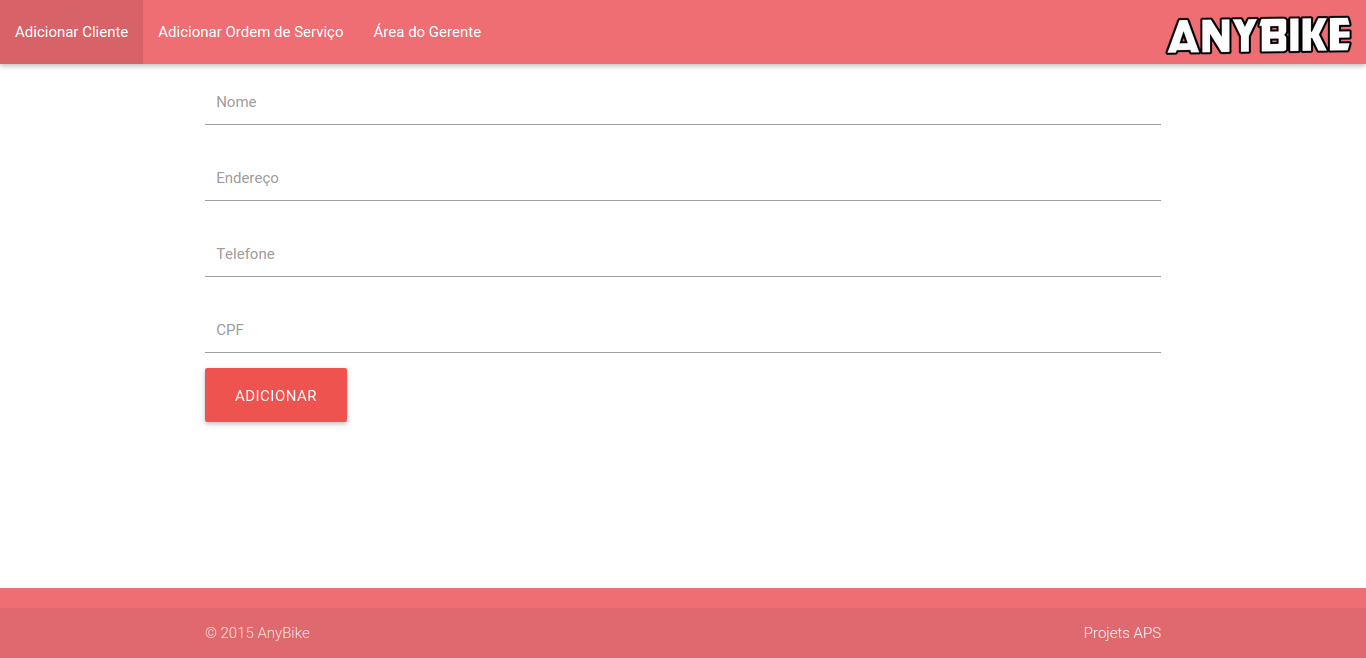
\includegraphics[scale=0.3]{Arquivos/adicionar_cliente}  
	\end{center}
	\legend{Fonte:Elaborado pelo autor}
\end{figure}


\begin{figure}[htb]
	\caption{Tela de adicionar funcionário}
	\begin{center}
	    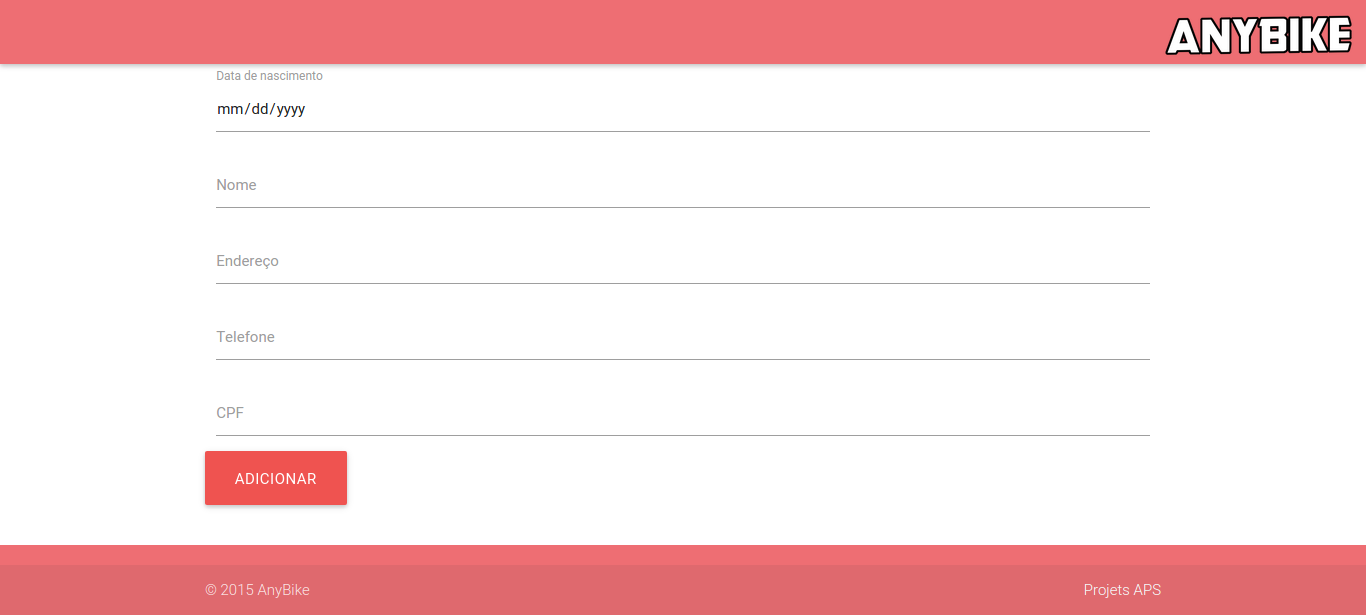
\includegraphics[scale=0.3]{Arquivos/adicionar_funcionario}  
	\end{center}
	\legend{Fonte:Elaborado pelo autor}
\end{figure}


\begin{figure}[htb]
	\caption{Tela de adicionar serviços oferecidos}
	\begin{center}
	    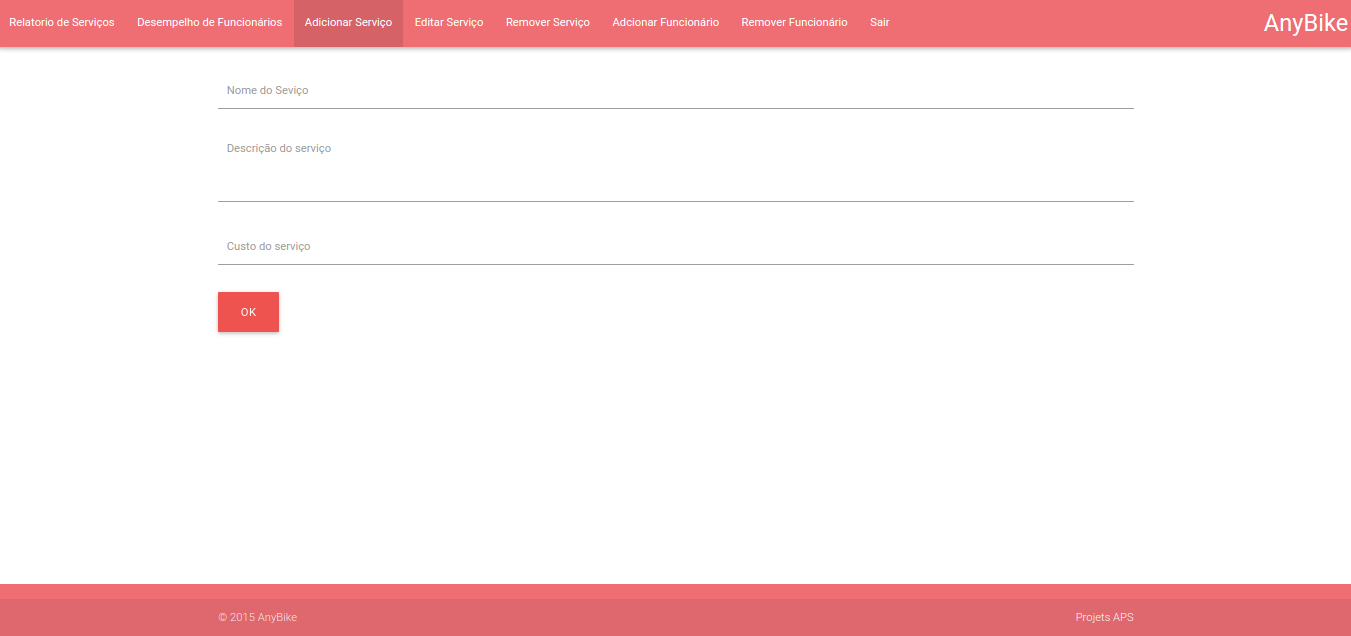
\includegraphics[scale=0.3]{Arquivos/adicionar_servico}  
	\end{center}
	\legend{Fonte:Elaborado pelo autor}
\end{figure}


\begin{figure}[htb]
	\caption{Tela de Cria uma ordem de serviço}
	\begin{center}
	    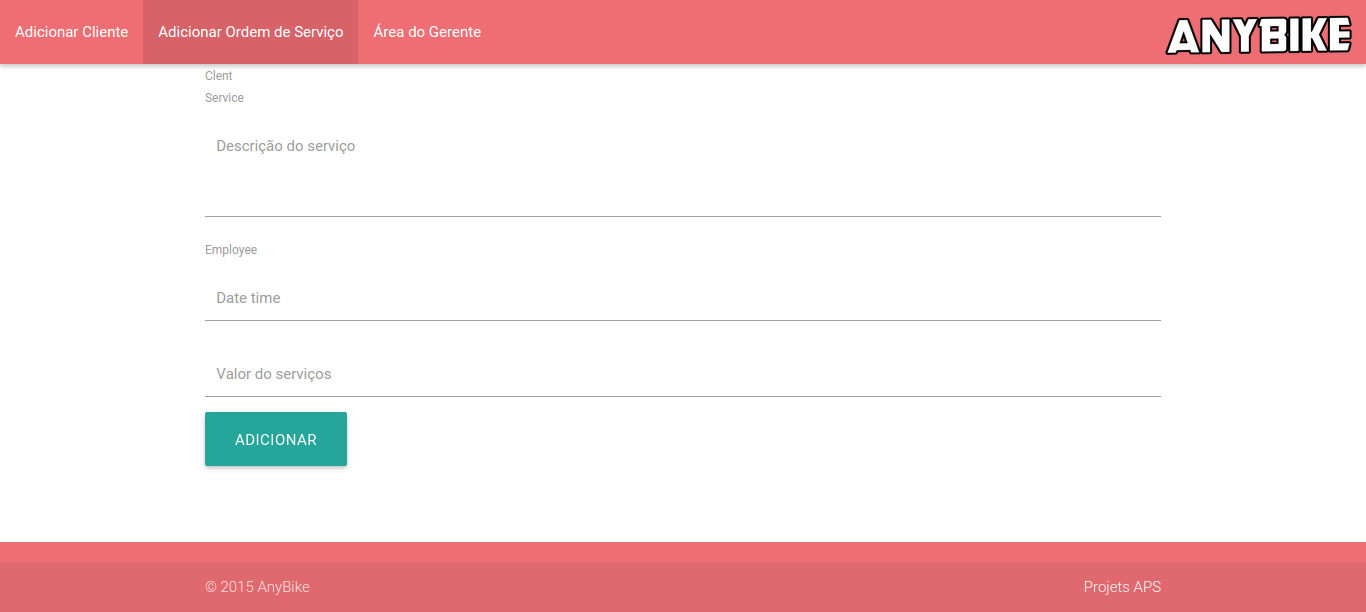
\includegraphics[scale=0.3]{Arquivos/ordem_servico}  
	\end{center}
	\legend{Fonte:Elaborado pelo autor}
\end{figure}


\begin{figure}[htb]
	\caption{Tela de login para o gerente}
	\begin{center}
	    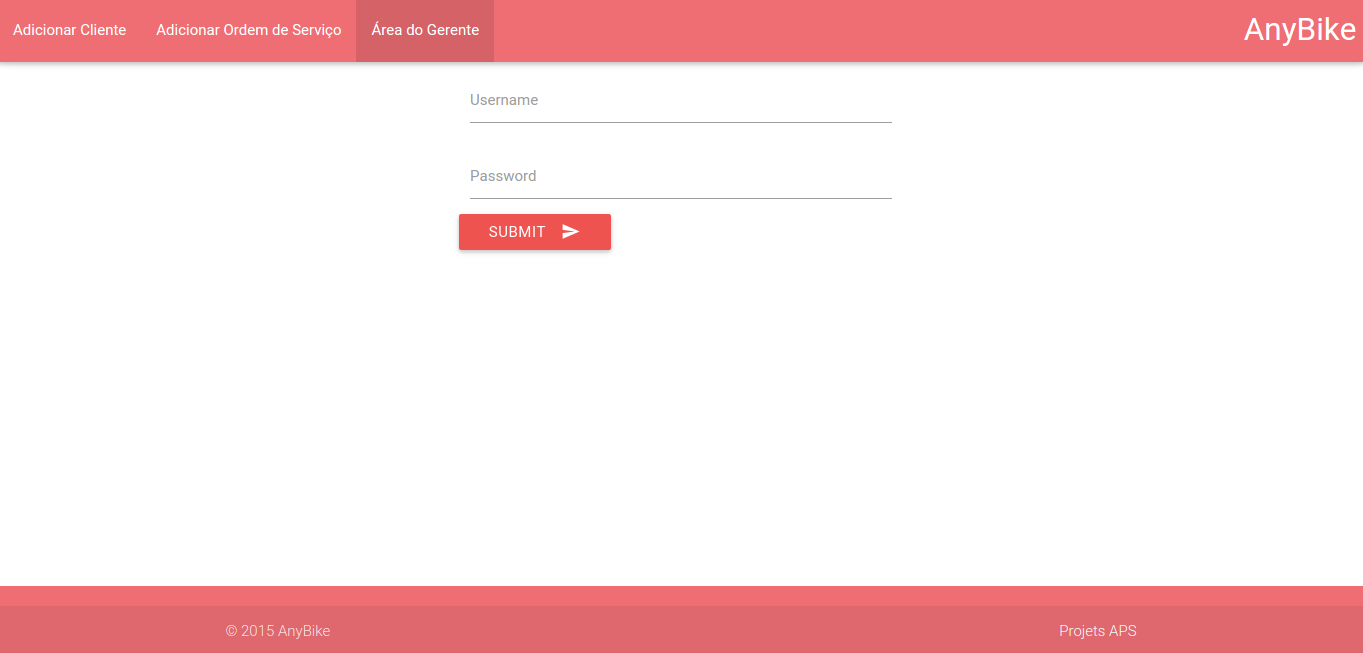
\includegraphics[scale=0.3]{Arquivos/login}  
	\end{center}
	\legend{Fonte:Elaborado pelo autor}
\end{figure}


\begin{figure}[htb]
	\caption{Tela que informa o desempenho dos funcionários}
	\begin{center}
	    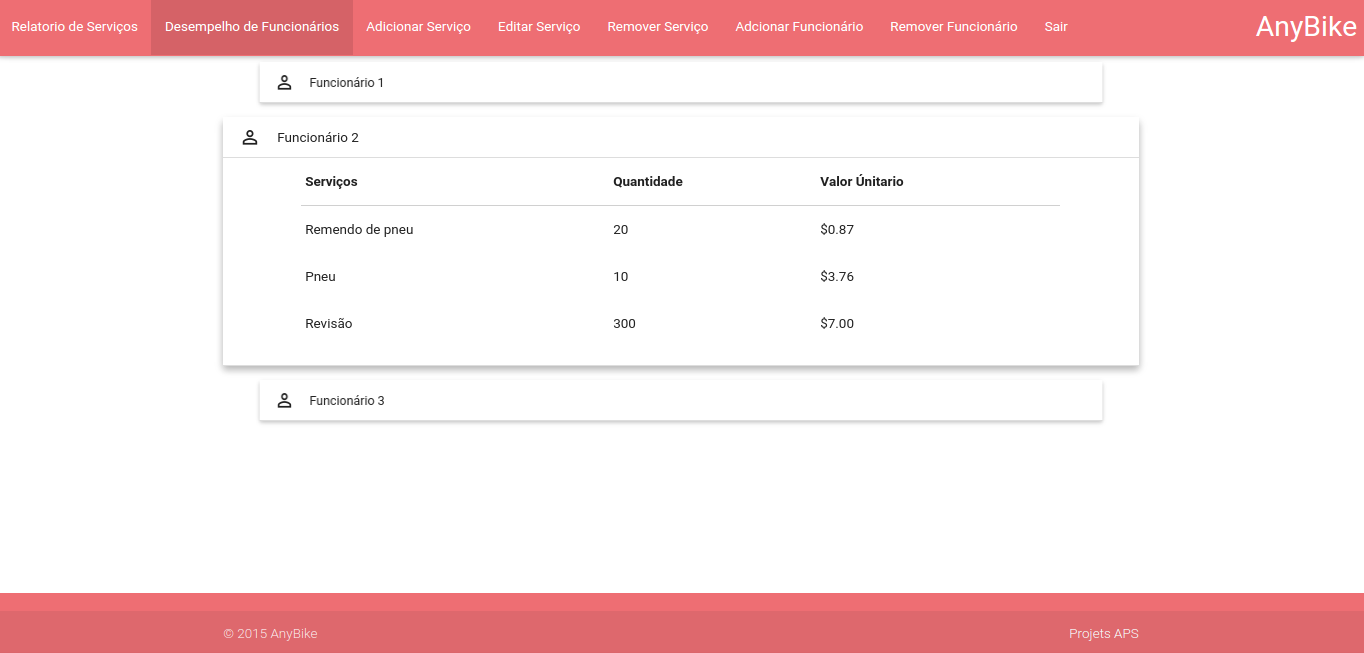
\includegraphics[scale=0.3]{Arquivos/relatorio_funcionario}  %TODO
	\end{center}
	\legend{Fonte:Elaborado pelo autor}
\end{figure}


\begin{figure}[htb]
	\caption{Tela que informa dados sobre cada serviço disponível}
	\begin{center}
	    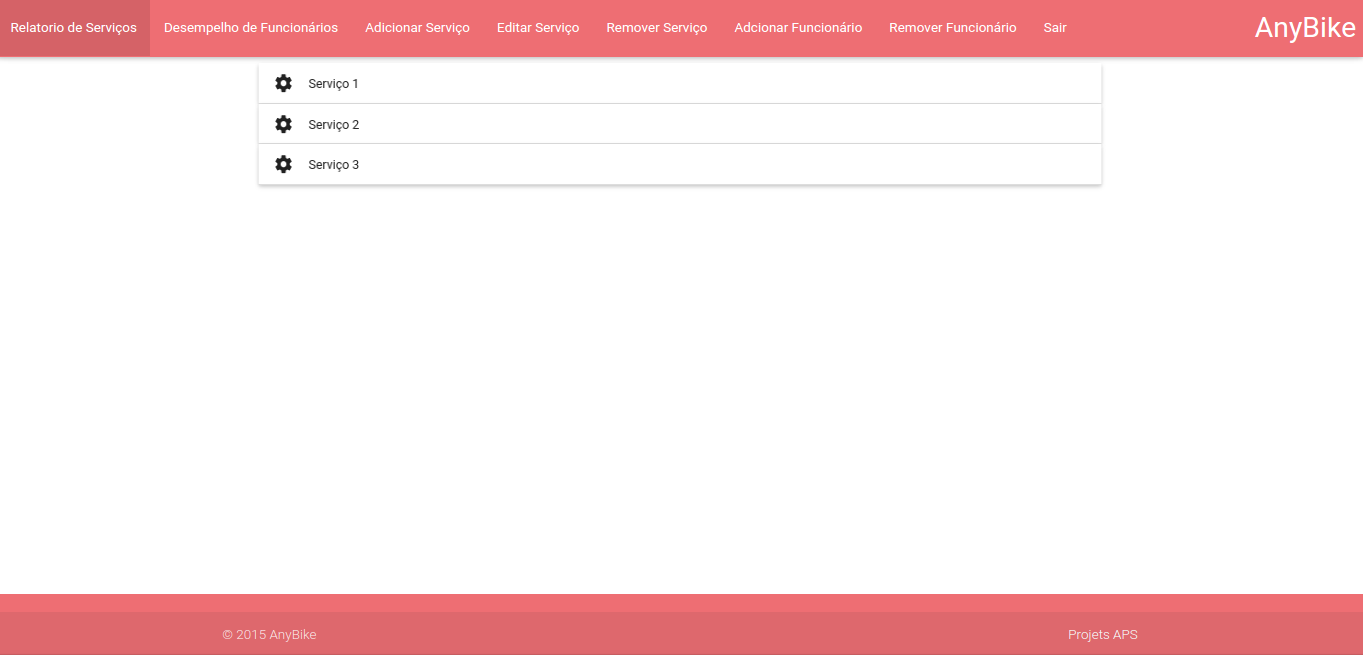
\includegraphics[scale=0.3]{Arquivos/relatorio_servico}  %TODO
	\end{center}
	\legend{Fonte:Elaborado pelo autor}
\end{figure}





\newpage
\chapter{Evolução do Sistema}

Após a construção e implantação do sistema, ele será acompanhado mensalmente. Esse acompanhamento prevê alterações necessárias para o bom funcionamento do sistema. Melhorias que possam vir a ser necessárias, como incremento de novos requisitos, passarão por um novo processo de desenvolvimento.
  

\end{document}

